%%
%% FSDP Benchmark Report - ACM sigconf format
%%
%TC:macro \cite [option:text,text]
%TC:macro \citep [option:text,text]
%TC:macro \citet [option:text,text]
%TC:envir table 0 1
%TC:envir table* 0 1
%TC:envir tabular [ignore] word
%TC:envir displaymath 0 word
%TC:envir math 0 word
%TC:envir comment 0 0
%%
\documentclass[sigconf]{acmart}

\AtBeginDocument{%
  \providecommand\BibTeX{{%
    Bib\TeX}}}

\setcopyright{none}
\settopmatter{printacmref=false, printfolios=true}
\renewcommand\footnotetextcopyrightpermission[1]{}
\pagestyle{plain}

\begin{document}

\title{Benchmarking PyTorch FSDP: Memory-Efficient Distributed Training for Vision Models}

\author{Shanzita Siddiqua}
\email{ss516@rice.edu}
\affiliation{%
  \institution{Rice University}
  \city{Houston}
  \state{Texas}
  \country{USA}}

\renewcommand{\shortauthors}{Siddiqua}

\begin{abstract}
Training large deep learning models is increasingly constrained by GPU memory capacity. Fully Sharded Data Parallel (FSDP) addresses this by sharding model parameters, gradients, and optimizer states across GPUs, enabling training of models that exceed single-GPU memory. We present a comprehensive benchmark comparing FSDP against single-GPU and DistributedDataParallel (DDP) training across 10 configurations, two vision models (ResNet-50 with 25.6M parameters and ViT-B/16 with 86.6M parameters), and multiple optimization techniques including mixed precision, activation checkpointing, CPU offloading, and gradient accumulation. On NVIDIA L40S GPUs, FSDP with mixed precision and activation checkpointing achieves up to 82\% memory reduction (from 5.16\,GB to 0.92\,GB per GPU for ViT-B/16) while FSDP with mixed precision alone delivers 2.3$\times$ higher throughput than single-GPU training. Our GPU scaling study shows DDP achieves 95--97\% scaling efficiency versus 82--94\% for FSDP, quantifying the communication overhead introduced by parameter sharding. Batch size scaling experiments reveal that FSDP with mixed precision reaches peak throughput of 1472 samples/sec at batch size 128 for ViT-B/16, 3.2$\times$ higher than DDP's peak. We provide practical guidelines for selecting FSDP configurations based on memory and throughput requirements.
\end{abstract}

\begin{CCSXML}
<ccs2012>
 <concept>
  <concept_id>10010147.10010169.10010170</concept_id>
  <concept_desc>Computing methodologies~Parallel computing methodologies</concept_desc>
  <concept_significance>500</concept_significance>
 </concept>
 <concept>
  <concept_id>10010147.10010257.10010293.10010294</concept_id>
  <concept_desc>Computing methodologies~Neural networks</concept_desc>
  <concept_significance>300</concept_significance>
 </concept>
 <concept>
  <concept_id>10010520.10010521.10010537.10010540</concept_id>
  <concept_desc>Computer systems organization~GPU computing</concept_desc>
  <concept_significance>300</concept_significance>
 </concept>
</ccs2012>
\end{CCSXML}

\ccsdesc[500]{Computing methodologies~Parallel computing methodologies}
\ccsdesc[300]{Computing methodologies~Neural networks}
\ccsdesc[300]{Computer systems organization~GPU computing}

\keywords{distributed training, FSDP, data parallelism, memory optimization, GPU benchmarking, mixed precision, activation checkpointing}

\begin{teaserfigure}
  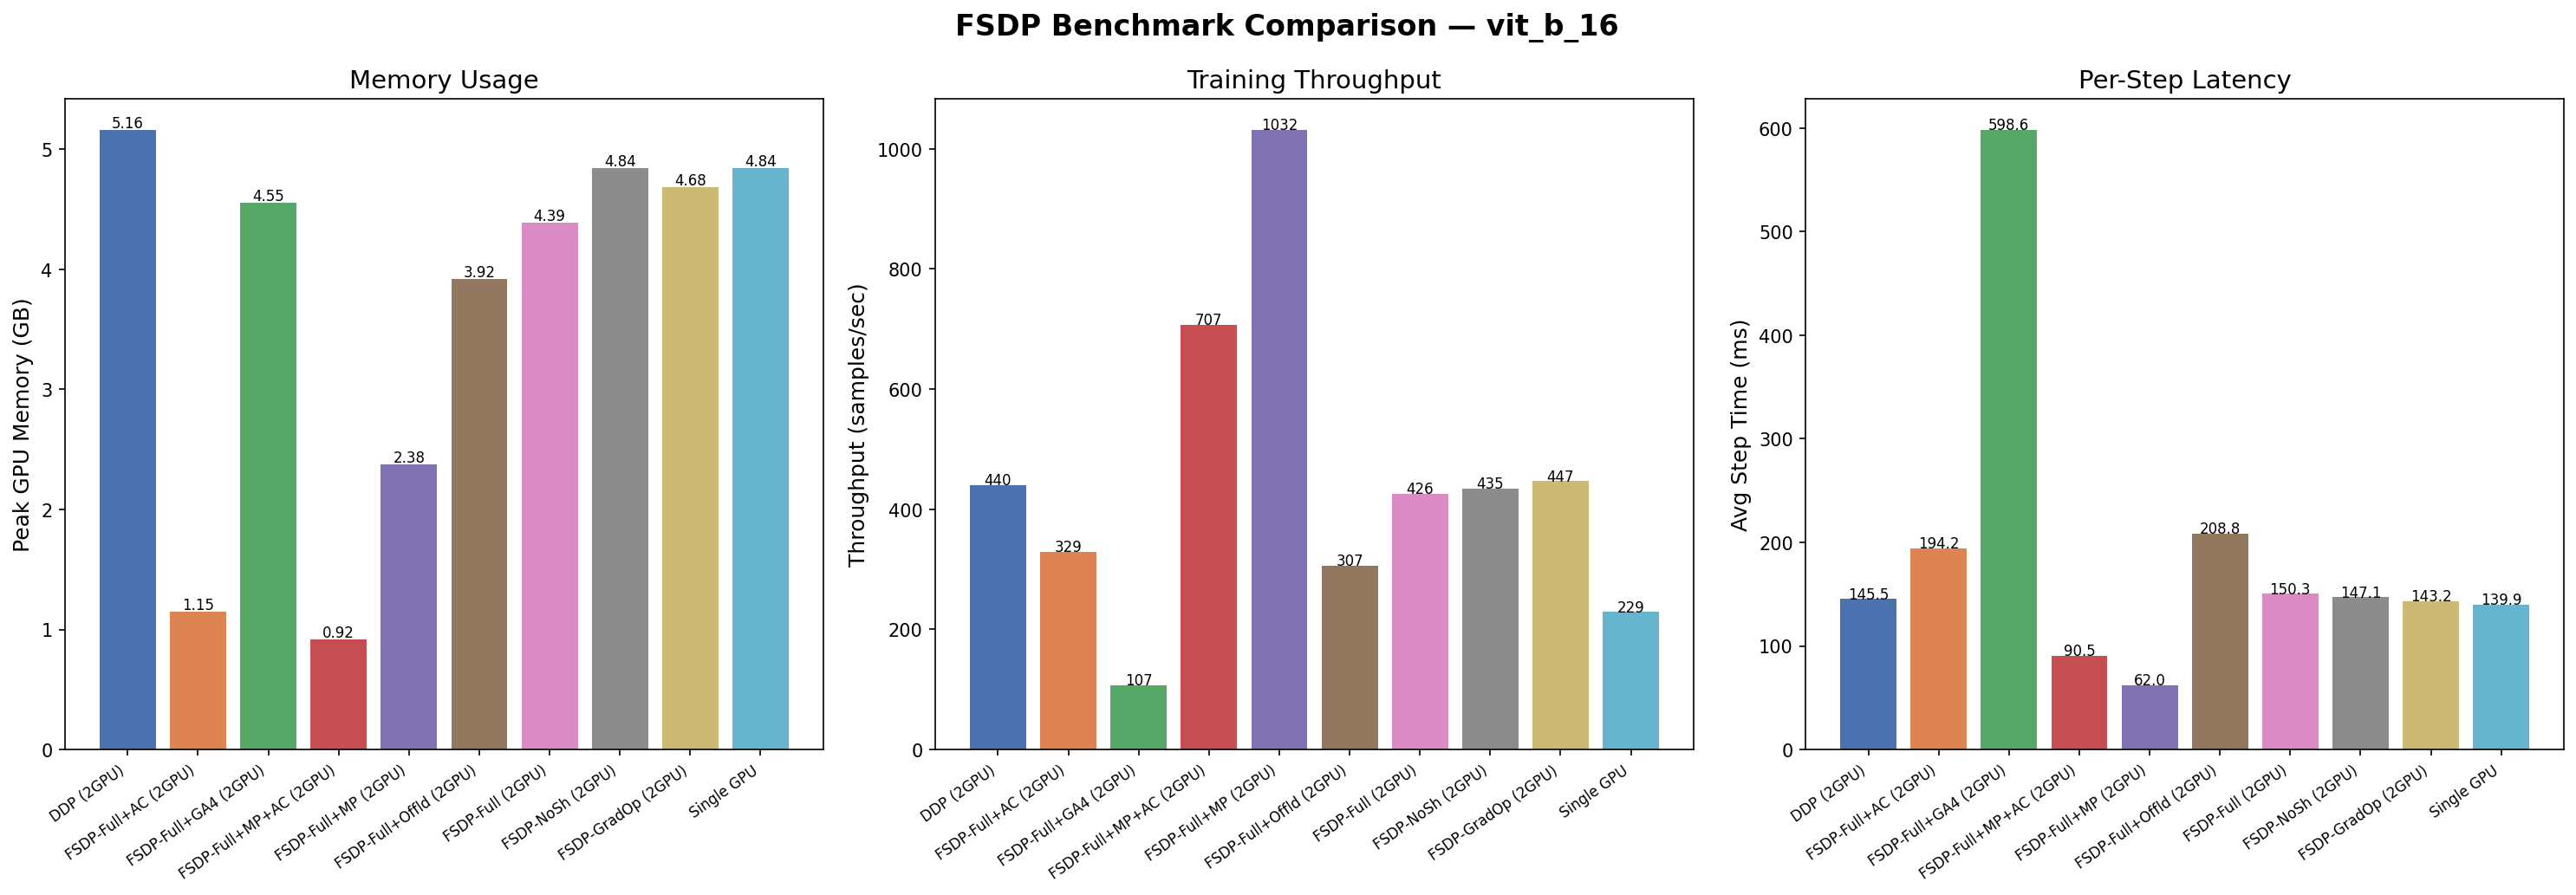
\includegraphics[width=\textwidth]{fig_comparison_vit_b_16.png}
  \caption{FSDP benchmark comparison for ViT-B/16 (86.6M parameters) across 10 training configurations on 2$\times$ NVIDIA L40S GPUs. Left: peak GPU memory usage; Center: training throughput; Right: per-step latency. FSDP with mixed precision achieves the highest throughput (1032\,samples/sec) while FSDP+MP+AC achieves the lowest memory (0.92\,GB per GPU).}
  \Description{Three bar charts comparing memory usage, throughput, and latency across 10 distributed training configurations for the ViT-B/16 vision transformer model. The charts show that FSDP with mixed precision and activation checkpointing reduces memory by 82 percent compared to DDP.}
  \label{fig:teaser}
\end{teaserfigure}

%%\received{5 May 2026}

\maketitle

\section{Introduction}

The rapid growth of deep learning model sizes has created a fundamental tension between model capacity and GPU memory. While models like Vision Transformers~\cite{dosovitskiy2021vit} achieve state-of-the-art accuracy, their parameter counts (86M--304M+ parameters) strain GPU memory during training due to the need to store model parameters, gradients, optimizer states, and activations simultaneously.

DistributedDataParallel (DDP)~\cite{li2020ddp} is the standard approach for multi-GPU training in PyTorch~\cite{paszke2019pytorch}, replicating the full model on each GPU and synchronizing gradients via all-reduce. While DDP provides near-linear throughput scaling, it does not reduce per-GPU memory usage---each GPU must hold the entire model, optimizer states, and gradients.

Fully Sharded Data Parallel (FSDP)~\cite{zhao2023fsdp}, inspired by ZeRO~\cite{rajbhandari2020zero}, addresses this limitation by \emph{sharding} parameters, gradients, and optimizer states across GPUs. Parameters are gathered on-demand for computation and released afterward, trading communication overhead for memory savings. FSDP supports multiple sharding strategies and can be combined with mixed precision training~\cite{micikevicius2018mixed}, activation checkpointing~\cite{chen2016checkpointing}, and CPU offloading to further reduce memory requirements.

Despite the importance of these techniques, there is limited empirical guidance on the quantitative tradeoffs between FSDP configurations. In this work, we present a systematic benchmark evaluating 10 training configurations across two vision models on NVIDIA L40S GPUs, measuring throughput, memory usage, and scaling efficiency. Our contributions are:

\begin{itemize}
  \item We show that FSDP with mixed precision \emph{Pareto-dominates} DDP on transformer training, achieving 54\% lower memory and 2.3$\times$ higher throughput simultaneously---contradicting the common assumption that FSDP trades speed for memory.
  \item We quantify the multiplicative benefit of stacking memory optimizations: combining FSDP sharding, mixed precision, and activation checkpointing yields 82\% memory reduction (5.16\,GB $\to$ 0.92\,GB per GPU for ViT-B/16).
  \item We measure GPU scaling efficiency and find FSDP's communication overhead is model-size-dependent: 81.8\% efficiency for ResNet-50 (25.6M params) vs.\ 93.6\% for ViT-B/16 (86.6M params), showing FSDP is best suited for larger models.
  \item We demonstrate through batch size sweeps that FSDP+MP enables 3.2$\times$ higher peak throughput than DDP (1472 vs.\ 460\,s/s for ViT-B/16) by unlocking larger optimal batch sizes.
\end{itemize}

\section{Experimental Setup}

\subsection{Models}

We evaluate two vision models from TorchVision: \textbf{ResNet-50}~\cite{he2016resnet} (25.6M parameters), a convolutional architecture, and \textbf{ViT-B/16}~\cite{dosovitskiy2021vit} (86.6M parameters), a transformer-based architecture. For OOM testing, we additionally use \textbf{ViT-L/16} (304M parameters). All models are trained on synthetic 224$\times$224 RGB data with random labels (1000 classes) to isolate computation from I/O effects.

\subsection{Hardware and Software}

Experiments run on a single node of the Rice University NOTS cluster with 2$\times$ NVIDIA L40S GPUs (44.3\,GB VRAM each), Intel Xeon Platinum 8468 CPU, PyTorch 2.5.1 with CUDA 12.1, and NCCL 2.21.5 for inter-GPU communication via shared memory (SHM/direct).

\subsection{Training Configuration}

All benchmarks use Adam optimizer (lr=$10^{-3}$), CrossEntropyLoss, batch size 32 per GPU, 5 warmup steps followed by 50 measured steps. FSDP uses a size-based auto-wrap policy with a 1M parameter threshold. Mixed precision uses FP16 parameters with FP32 reduction and buffers. Peak GPU memory is measured after warmup reset to exclude initialization costs.

\subsection{Configurations Evaluated}

Table~\ref{tab:configs} summarizes the 10 training configurations benchmarked in this study.

\begin{table}[h]
\caption{Training configurations evaluated. Each targets a different point in the memory--throughput tradeoff space.}
\label{tab:configs}
\small
\begin{tabular}{lll}
\toprule
\textbf{Configuration} & \textbf{Description} & \textbf{Optimizes} \\
\midrule
Single GPU & No distribution & Baseline \\
DDP (2 GPU) & Gradient all-reduce & Throughput \\
FSDP Full & Shard params/grads/optim & Memory \\
FSDP GradOp & Shard grads + optim only & Both \\
FSDP NoShard & No sharding (FSDP API) & Baseline \\
FSDP + MP & Full shard + FP16 & Both \\
FSDP + AC & Full shard + recompute acts & Memory \\
FSDP + MP + AC & Full shard + MP + AC & Memory \\
FSDP + Offload & Full shard + CPU offload & Memory \\
FSDP + GA4 & Full shard + 4$\times$ accum & Batch size \\
\bottomrule
\end{tabular}
\end{table}

\section{Results}

\subsection{Core Benchmark Comparison}

Table~\ref{tab:results} presents the complete benchmark results for both models across all 10 configurations, sorted by peak memory usage.

\begin{table*}[t]
\caption{Complete benchmark results for ResNet-50 (25.6M params) and ViT-B/16 (86.6M params) on 2$\times$ NVIDIA L40S GPUs. Configurations sorted by memory. Bold indicates best throughput and lowest memory per model.}
\label{tab:results}
\small
\begin{tabular}{l r r r r r r}
\toprule
& \multicolumn{3}{c}{\textbf{ResNet-50}} & \multicolumn{3}{c}{\textbf{ViT-B/16}} \\
\cmidrule(lr){2-4} \cmidrule(lr){5-7}
\textbf{Configuration} & \textbf{Step (ms)} & \textbf{Thru (s/s)} & \textbf{Mem (GB)} & \textbf{Step (ms)} & \textbf{Thru (s/s)} & \textbf{Mem (GB)} \\
\midrule
Single GPU         &  43.58 &  734.2 & 2.919 & 139.86 &  228.8 & 4.844 \\
DDP (2GPU)         &  47.86 & 1337.2 & 3.018 & 145.48 &  439.9 & 5.164 \\
\midrule
FSDP Full          &  54.81 & 1167.7 & 2.783 & 150.27 &  425.9 & 4.391 \\
FSDP GradOp        &  47.29 & \textbf{1353.3} & 2.857 & 143.25 &  446.8 & 4.681 \\
FSDP NoShard       &  47.63 & 1343.7 & 2.923 & 147.14 &  435.0 & 4.845 \\
FSDP + MP          &  90.74 &  705.3 & 2.200 &  62.00 & \textbf{1032.2} & 2.377 \\
FSDP + AC          &  78.08 &  819.7 & 1.246 & 194.24 &  329.5 & 1.151 \\
FSDP + Offload     &  82.23 &  778.3 & 2.640 & 208.76 &  306.6 & 3.919 \\
FSDP + GA4         & 217.35 &  294.5 & 2.826 & 598.59 &  106.9 & 4.552 \\
FSDP + MP + AC     & 136.70 &  468.2 & \textbf{1.001} &  90.53 &  706.9 & \textbf{0.917} \\
\bottomrule
\end{tabular}
\end{table*}

\textbf{Sharding strategies.} Among the three FSDP sharding strategies, FULL\_SHARD provides the greatest memory reduction (4.39\,GB vs.\ 5.16\,GB for DDP on ViT-B/16, a 15\% saving) but incurs a 3.2\% throughput penalty (426 vs.\ 440\,s/s) due to additional all-gather and reduce-scatter communication. SHARD\_GRAD\_OP offers a middle ground with 9.4\% memory savings and the highest throughput among all FSDP configurations (447\,s/s for ViT-B/16). NO\_SHARD, as expected, matches DDP's memory footprint and performance, confirming it acts as a DDP-equivalent wrapper.

\textbf{Mixed precision.} FSDP+MP dramatically improves both memory and throughput for ViT-B/16: memory drops to 2.38\,GB (54\% reduction vs.\ DDP) while throughput \emph{increases} to 1032\,s/s---2.3$\times$ faster than single GPU and 2.4$\times$ faster than FSDP without MP. This occurs because L40S GPUs have dedicated FP16 tensor cores that accelerate half-precision computation, and the reduced parameter size decreases communication volume.

\textbf{Activation checkpointing.} FSDP+AC reduces memory to 1.15\,GB for ViT-B/16 (78\% reduction vs.\ DDP) by recomputing activations during the backward pass instead of storing them. However, this recomputation introduces a significant throughput penalty: 329\,s/s (25\% slower than FSDP alone).

\textbf{Combined MP+AC.} Stacking both optimizations yields the minimum memory footprint: \textbf{0.92\,GB} for ViT-B/16, an \textbf{82\% reduction} from DDP's 5.16\,GB. Throughput remains competitive at 707\,s/s---still 3.1$\times$ faster than single GPU training.

\textbf{CPU offloading.} FSDP+Offload reduces GPU memory to 3.92\,GB but incurs the largest throughput penalty (307\,s/s, 28\% slower than FSDP alone), making it the least favorable option when GPU memory is sufficient.

\textbf{Gradient accumulation.} FSDP+GA4 simulates a 4$\times$ larger effective batch size (256 total) without additional memory for larger batches. Per-step time increases proportionally ($\sim$4$\times$) as expected, while memory remains comparable to standard FSDP.

\subsection{Memory--Throughput Tradeoff}

Figure~\ref{fig:tradeoff} visualizes the Pareto frontier of memory vs.\ throughput across all configurations and models. The ideal operating point is the upper-left corner (low memory, high throughput).

\begin{figure}[h]
  \centering
  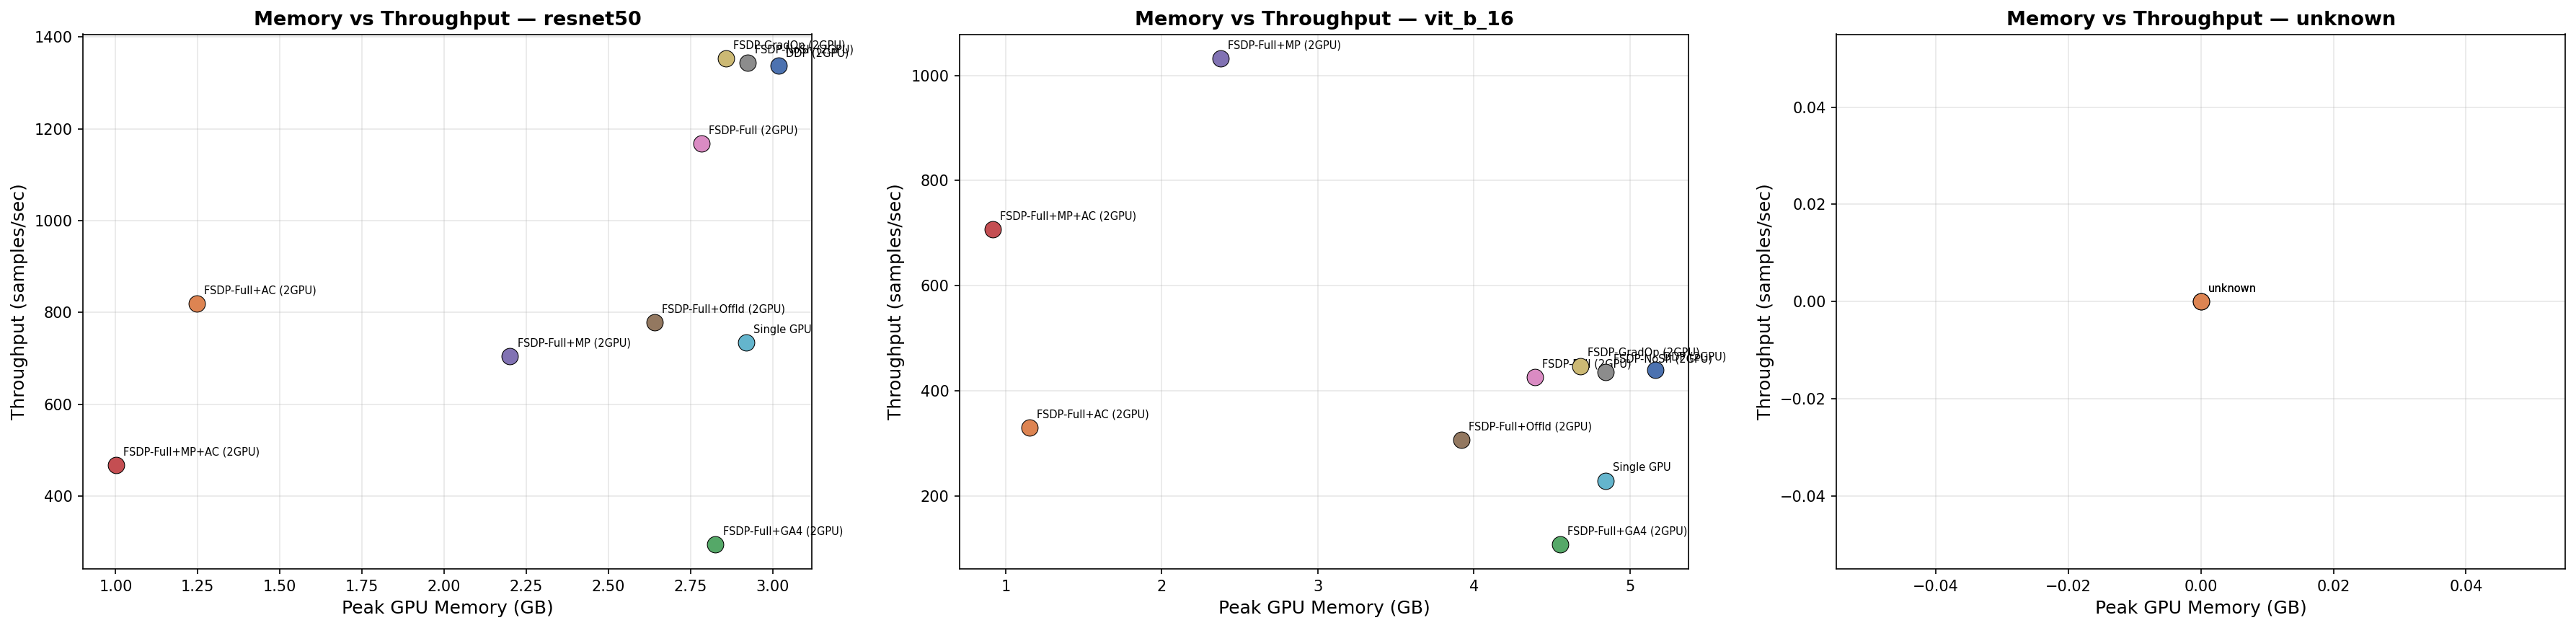
\includegraphics[width=\columnwidth]{fig_tradeoff.png}
  \caption{Memory vs.\ throughput tradeoff across all configurations and both models. The ideal operating point is the upper-left (low memory, high throughput). FSDP+MP for ViT-B/16 Pareto-dominates DDP---it uses 54\% less memory (2.38 vs.\ 5.16\,GB) \emph{and} delivers 2.3$\times$ higher throughput (1032 vs.\ 440\,s/s), contradicting the assumption that memory savings require a speed penalty.}
  \Description{Scatter plot with peak GPU memory on x-axis and throughput on y-axis. Each point represents a training configuration. FSDP with mixed precision for ViT-B/16 appears in the upper-left, indicating it is Pareto-optimal.}
  \label{fig:tradeoff}
\end{figure}

A key finding is that FSDP+MP for ViT-B/16 \emph{Pareto-dominates} DDP: it uses less memory (2.38 vs.\ 5.16\,GB) \emph{and} delivers higher throughput (1032 vs.\ 440\,s/s). This dominance occurs because the FP16 computation speedup from tensor cores more than compensates for FSDP's communication overhead.

\subsection{Memory Reduction Analysis}

Figure~\ref{fig:waterfall} ranks all configurations by memory usage for ViT-B/16, showing the progressive reduction achieved by stacking optimization techniques.

\begin{figure}[h]
  \centering
  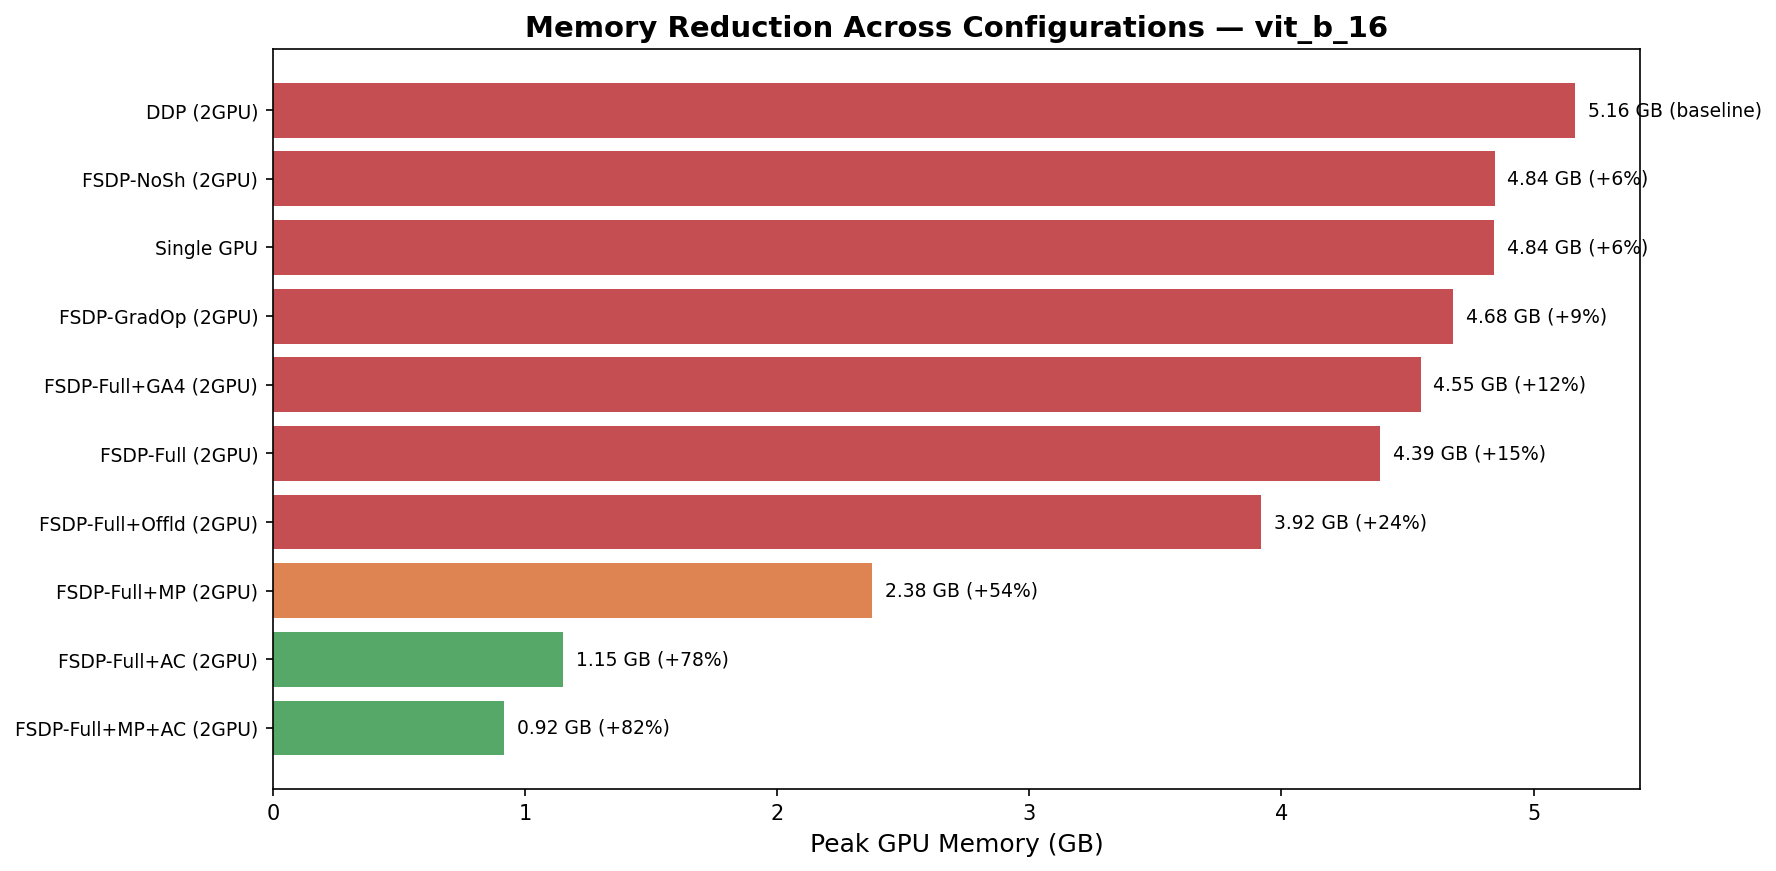
\includegraphics[width=\columnwidth]{fig_memory_waterfall_vit_b_16.png}
  \caption{Memory reduction waterfall for ViT-B/16. Configurations ranked by peak GPU memory with percentage reduction from the DDP baseline (5.16\,GB).}
  \Description{Horizontal bar chart ranking all configurations from highest to lowest memory usage for ViT-B/16. DDP uses the most memory at 5.16 GB and FSDP+MP+AC uses the least at 0.92 GB.}
  \label{fig:waterfall}
\end{figure}

The waterfall reveals a clear hierarchy of memory optimization techniques: sharding alone provides 15\% reduction, mixed precision adds another 39\%, and activation checkpointing contributes an additional 28\%. The combined effect is multiplicative rather than additive, achieving 82\% total reduction.

\subsection{GPU Scaling Efficiency}

Figure~\ref{fig:scaling} shows throughput, scaling efficiency, and per-GPU memory from 1 to 2 GPUs for both DDP and FSDP on ViT-B/16.

\begin{figure}[h]
  \centering
  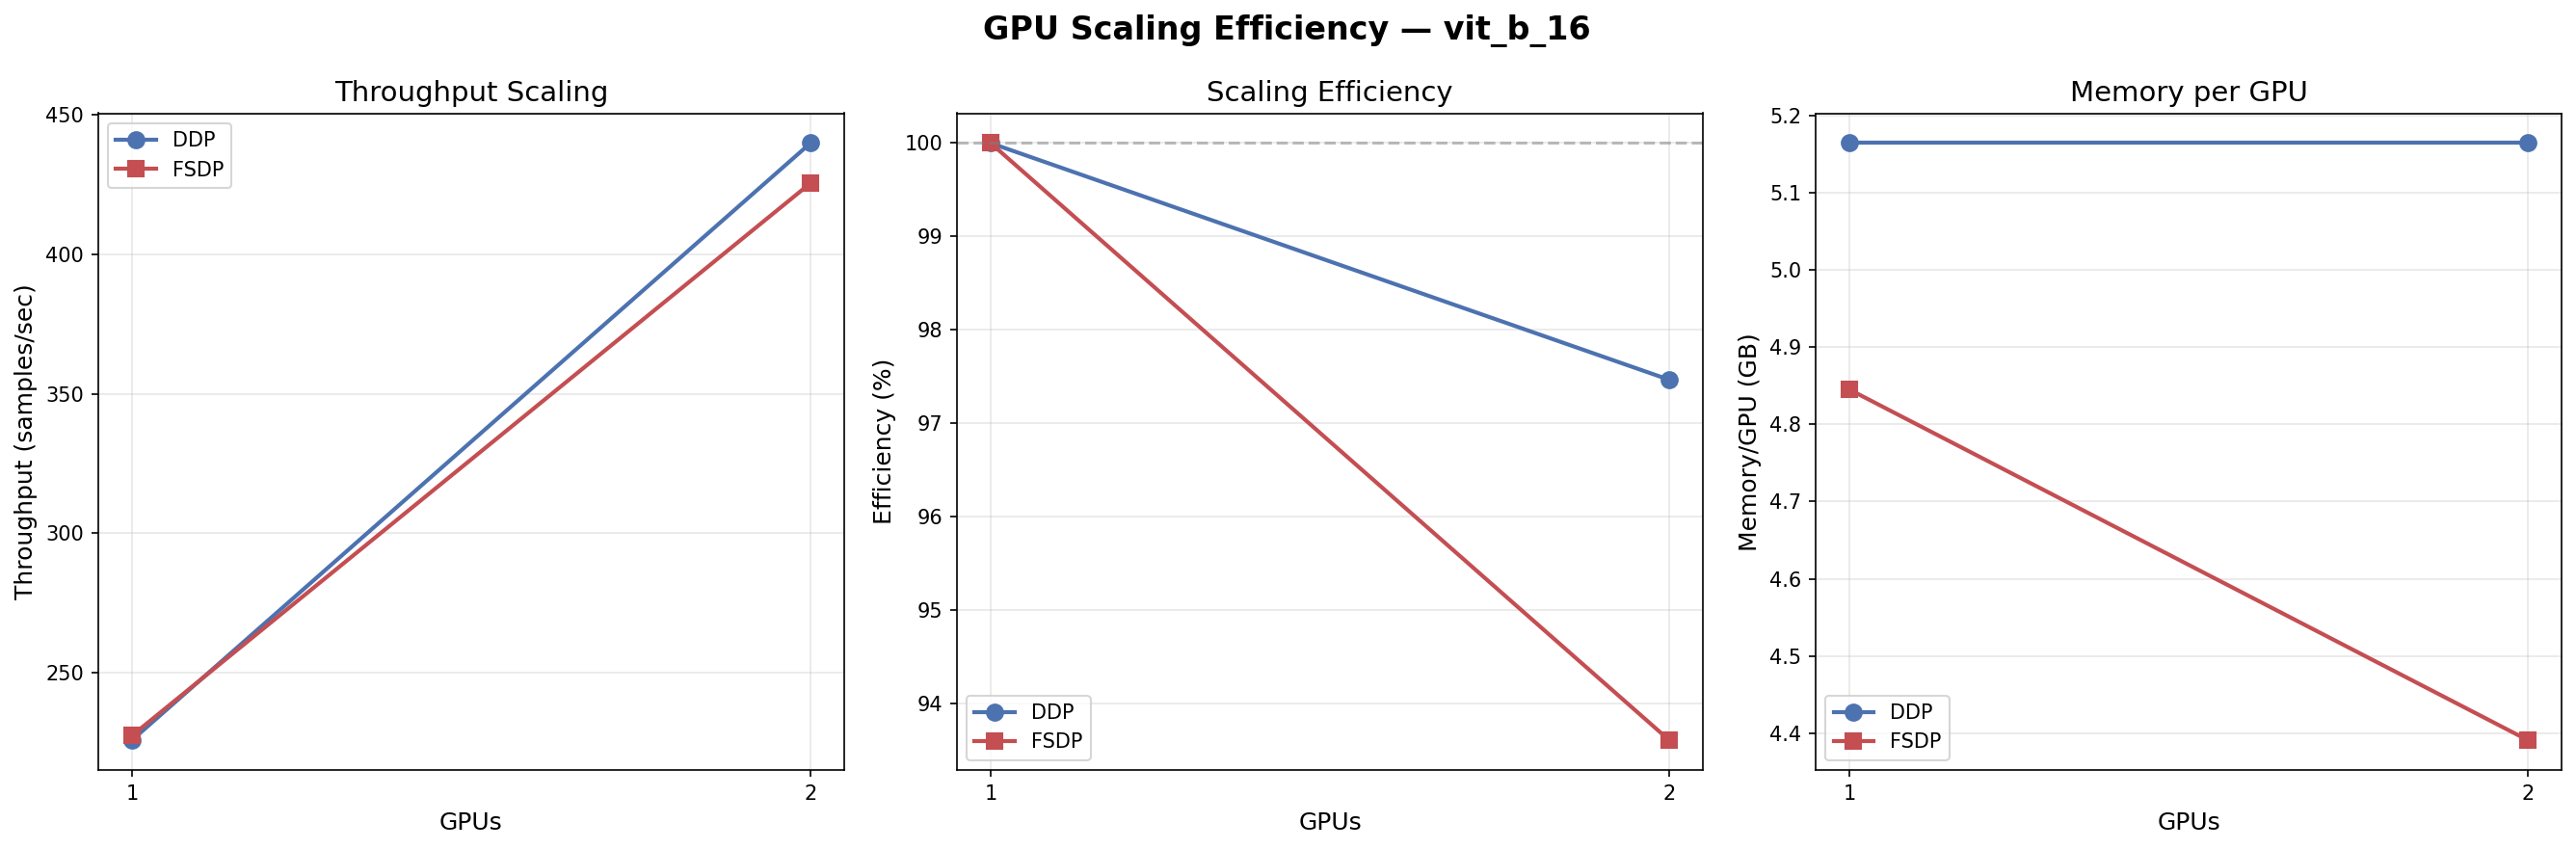
\includegraphics[width=\columnwidth]{fig_scaling_vit_b_16.png}
  \caption{GPU scaling analysis for ViT-B/16. DDP achieves 97.5\% efficiency versus 93.6\% for FSDP. FSDP uses 9.4\% less memory per GPU while maintaining competitive scaling.}
  \Description{Three line plots comparing DDP and FSDP scaling from 1 to 2 GPUs. Left plot shows throughput increasing for both. Center plot shows DDP at 97.5 percent efficiency and FSDP at 93.6 percent. Right plot shows FSDP using less memory per GPU.}
  \label{fig:scaling}
\end{figure}

DDP achieves 95.0--97.5\% scaling efficiency (ResNet-50 and ViT-B/16 respectively), while FSDP achieves 81.8--93.6\%. The lower FSDP efficiency for ResNet-50 (81.8\%) reflects the higher communication-to-computation ratio for smaller models: the all-gather and reduce-scatter operations become a larger fraction of total step time. For the larger ViT-B/16, FSDP's efficiency improves to 93.6\% as computation dominates communication, suggesting FSDP's overhead is better amortized for larger models---precisely the regime where its memory savings are most needed.

\subsection{Batch Size Scaling}

Figure~\ref{fig:batch} shows how throughput and memory scale with batch size (8 to 256) across single-GPU, DDP, FSDP, and FSDP+MP for ViT-B/16.

\begin{figure}[h]
  \centering
  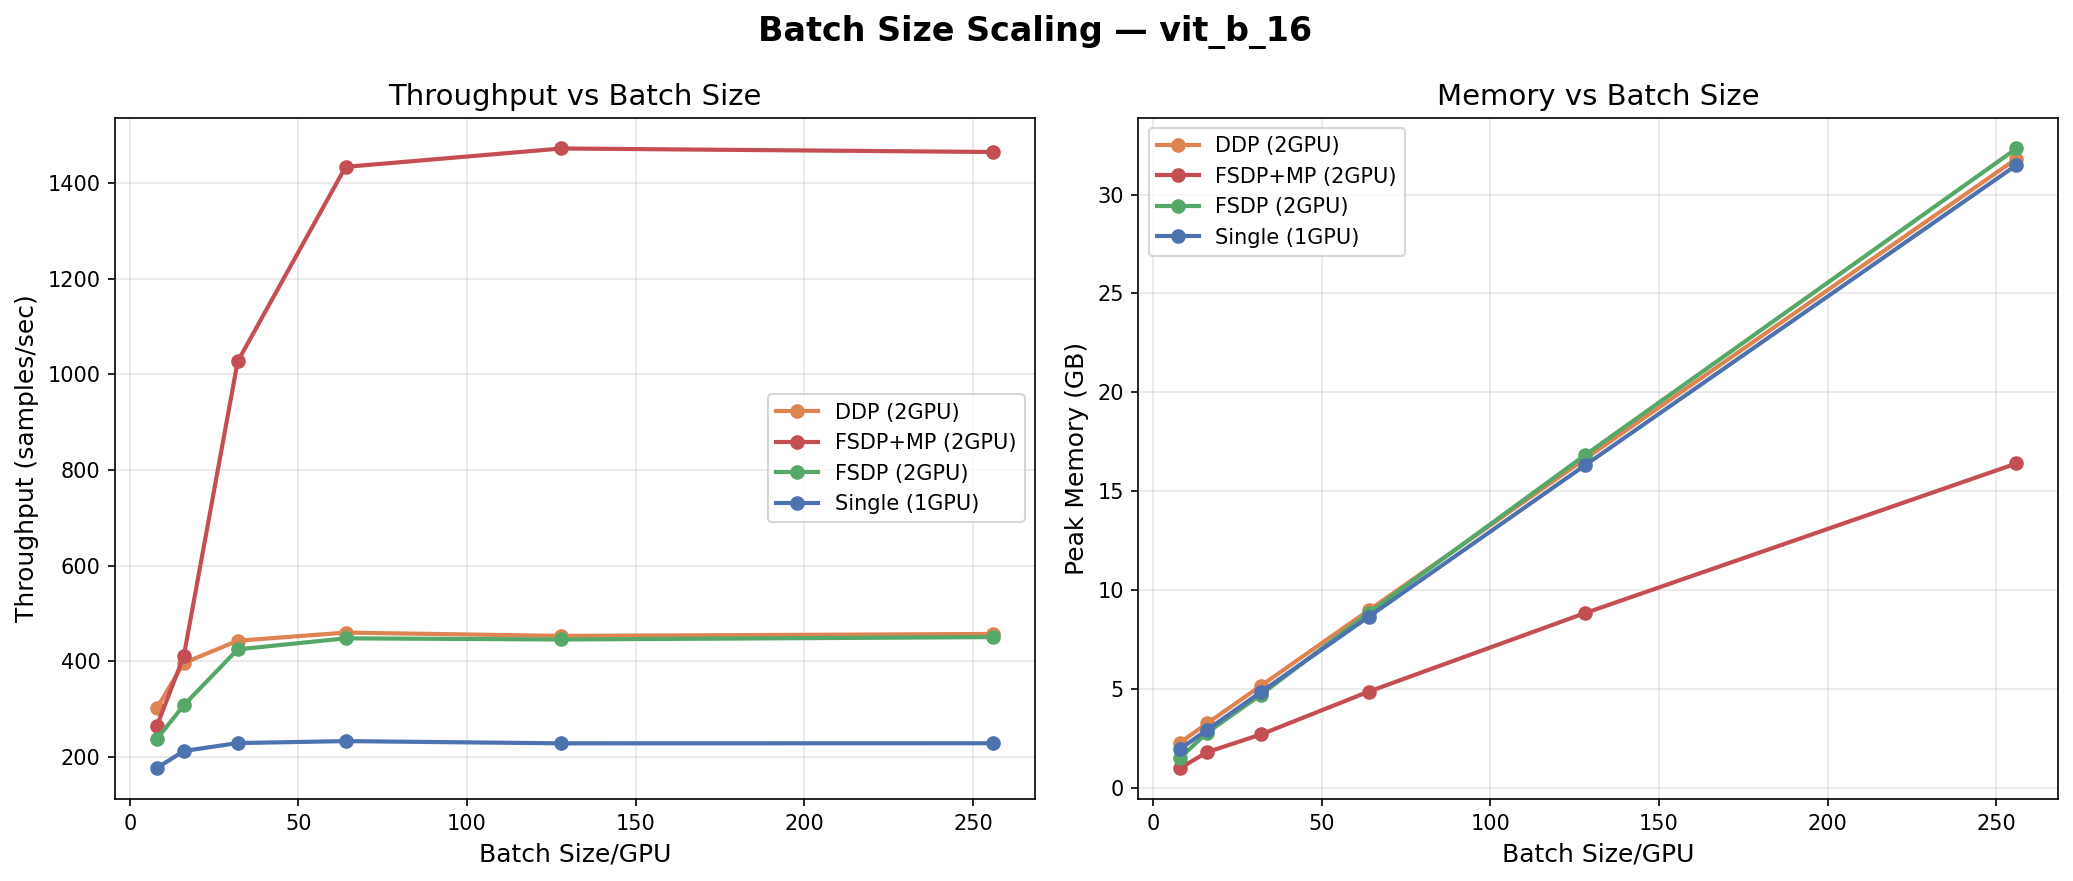
\includegraphics[width=\columnwidth]{fig_batch_scaling_vit_b_16.png}
  \caption{Batch size scaling for ViT-B/16. FSDP+MP peaks at 1472\,s/s (bs=128), 3.2$\times$ higher than DDP's peak of 460\,s/s (bs=64). All configurations fit up to bs=256 on the 44.3\,GB L40S GPUs.}
  \Description{Two line plots showing throughput and memory versus batch size. FSDP+MP achieves significantly higher throughput at all batch sizes compared to other configurations. Memory grows linearly with batch size for all configurations.}
  \label{fig:batch}
\end{figure}

FSDP+MP with ViT-B/16 peaks at 1472\,s/s (batch size 128), 3.2$\times$ faster than DDP's peak of 460\,s/s (batch size 64). This advantage comes from FP16 halving the memory footprint of parameters and activations, combined with better tensor core utilization at larger batch sizes. On GPUs with less memory than the L40S's 44.3\,GB, FSDP's memory savings would enable batch sizes that cause out-of-memory errors on DDP.

\section{Discussion and Conclusion}

Our benchmark reveals several practical insights for practitioners selecting distributed training strategies:

\textbf{FSDP+MP is often the best default.} For transformer models on modern GPUs with tensor cores, FSDP with mixed precision provides a surprising result: it is both more memory-efficient \emph{and} faster than DDP, achieving Pareto dominance on both axes. This makes it the recommended default for transformer training.

\textbf{Activation checkpointing trades compute for memory.} AC reduces memory by 76--82\% but adds 25--45\% latency overhead from activation recomputation. It should be reserved for cases where models or batch sizes would otherwise cause out-of-memory errors.

\textbf{CPU offloading is a last resort.} Offloading parameters to CPU introduces the highest throughput penalty (28--37\% slower) with moderate memory savings, making it justified only when all other techniques are insufficient.

\textbf{Scaling efficiency improves with model size.} FSDP's communication overhead is better amortized for larger models (93.6\% efficiency for ViT-B/16 vs.\ 81.8\% for ResNet-50), suggesting FSDP becomes increasingly advantageous as model size grows.

\textbf{Sharding strategy selection.} SHARD\_GRAD\_OP offers the best throughput among FSDP strategies with moderate memory savings, while FULL\_SHARD maximizes memory reduction at a small throughput cost. NO\_SHARD provides no benefit over DDP.

In summary, we benchmarked 10 distributed training configurations across two vision models and found three key results: (1)~FSDP with mixed precision Pareto-dominates DDP for transformer models, achieving both lower memory and higher throughput; (2)~stacking FSDP sharding with mixed precision and activation checkpointing yields multiplicative memory savings of up to 82\%; and (3)~FSDP's scaling efficiency is model-size-dependent, reaching 93.6\% for ViT-B/16 versus 81.8\% for ResNet-50, confirming that FSDP's benefits grow with model size. These findings provide practitioners with concrete, data-driven guidance for selecting distributed training strategies.

\textbf{Limitations and future work.} Our study is limited to single-node, 2-GPU configurations and synthetic data. Multi-node training with network communication overhead, real data loading pipelines, and models exceeding 1B parameters would provide additional insights. Future work should evaluate PyTorch's next-generation FSDP2 implementation and compare against DeepSpeed ZeRO~\cite{rasley2020deepspeed} stages on identical hardware.

All benchmark code and results are publicly available at \url{https://github.com/Shanzita/fsdp-benchmark}.

\begin{acks}
Experiments were conducted on the NOTS cluster at Rice University using NVIDIA L40S GPUs. We thank the Rice Center for Research Computing for providing computational resources.
\end{acks}

\bibliographystyle{ACM-Reference-Format}
\bibliography{references}

\end{document}
